\documentclass[11pt, oneside]{article}   	% use "amsart" instead of "article" for AMSLaTeX format
\usepackage[margin=1in]{geometry}                		% See geometry.pdf to learn the layout options. There are lots.
\geometry{letterpaper}                   		% ... or a4paper or a5paper or ... 
%\geometry{landscape}                		% Activate for rotated page geometry
%\usepackage[parfill]{parskip}    		% Activate to begin paragraphs with an empty line rather than an indent
\usepackage{graphicx}				% Use pdf, png, jpg, or eps§ with pdflatex; use eps in DVI mode
								% TeX will automatically convert eps --> pdf in pdflatex		
\usepackage{amssymb}
\usepackage{courier}
%usepackage{undertilde}
\usepackage[numbered,framed]{matlab-prettifier}
\usepackage{framed}

\usepackage[T1]{fontenc}
\usepackage{mathtools}  % loads »amsmath«
\usepackage{physics}
\usepackage{listings}

\lstset{
  language=C,                % choose the language of the code
  numbers=left,                   % where to put the line-numbers
  stepnumber=1,                   % the step between two line-numbers.        
  numbersep=5pt,                  % how far the line-numbers are from the code
  backgroundcolor=\color{white},  % choose the background color. You must add \usepackage{color}
  showspaces=false,               % show spaces adding particular underscores
  showstringspaces=false,         % underline spaces within strings
  showtabs=false,                 % show tabs within strings adding particular underscores
  tabsize=2,                      % sets default tabsize to 2 spaces
  captionpos=b,                   % sets the caption-position to bottom
  breaklines=true,                % sets automatic line breaking
  breakatwhitespace=true,         % sets if automatic breaks should only happen at whitespace
  title=\lstname,                 % show the filename of files included with \lstinputlisting;
}

\setlength{\parskip}{0.5em}

%SetFonts
\newcommand\Rey{\mbox{\textit{Re}}}

\title{\vspace{-6ex}\large PHYS 516: Methods of Computational Physics \\
  \normalsize ASSIGNMENT 4- Molecular Dynamics Simulation}
\author{Anup V Kanale}
\date{\vspace{-3ex}\today}							% Activate to display a given date or no date

\begin{document}
\maketitle
\vspace{-2ex} The purpose of this assignment is to get familiar with basic concepts in ordinary differential equations using a simple molecular dynamics (MD) program, \textit{md.c}, as an example.
\vspace{-2ex}
\section{Liouville Theorem}
\vspace{-2ex} Here, we show that for a particle in 1-D space, the velocity Verlet algorithm exactly preserves the phase space volume for arbitrary time discretization unit, $\Delta$.

 Let $x$ be the position of the particle, $p = mv$ the momentum where, $m$ and $v$ are the mass and velocity of the particle. In the dimensionless form, $p = v$. Let the coordinate and momentum of the particle at time $t$ be $(x, p)$, and those at time $t + \Delta$ be $(x',p')$
 \begin{align}
  x' &= x + p \Delta + \frac{1}{2} a(x) + \Delta^2 \\
  p' &= p + \frac{a(x) + a(x')}{2} \Delta
 \end{align}

To show this, it is enough to show that the Jacobian of the transformation  $(x'(x, p), p'(x, p))$ is $1$, i.e. $ J = \left| \dfrac{\partial (x', p')} {\partial (x, p)} \right| = 1$. The derivatives are calculated from Eq (1) and (2) as follows:
 \begin{align*}
 \pdv{x'}{x} &= 1 \\
 \pdv{x'}{p} &= \Delta \\
 \pdv{p'}{x} &= 0 \\
 \pdv{p'}{p} &= 1
 \end{align*}

Therefore, the Jacobian is given by
 \begin{align}
 J &= \begin{vmatrix}
   \dfrac{\partial x'}{\partial x} & \dfrac{\partial p'} {\partial x} \\[2ex]
   \dfrac{\partial x'}{\partial p} & \dfrac{\partial p'}{\partial p}
   \end{vmatrix} \\[1ex]
   &= \begin{vmatrix}
   1 & 0 \\[1ex]
   \Delta & 1
 \end{vmatrix} \\[1ex]
  &= 0
 \end{align}
\pagebreak
 
\section{Comparison of Euler and Velocity-Verlet Algorithms}
\vspace{-2ex} Total energy of the system should be conserved. But due to numerical errors, energy conservation depends on the time-integration algorithm used. In this section, we illustrate this by comparing the Euler and Velocity-Verlet algorithms.
 
\begin{framed}
	\textbf{Euler Algorithm}
	
	Given a configuration ($\boldsymbol{r}_i(t), \boldsymbol{v}_i(t) | i = 1$ to $N_{atom}$)
	
	1. Compute the acceleration: $\boldsymbol{a}_i(t)$
	
	2. Update the positions: $\boldsymbol{r}_i(t + \Delta) \leftarrow \boldsymbol{r}_i(t) + \boldsymbol{v}_i(t) \Delta + \frac{1}{2}\boldsymbol{a}_i(t) \Delta^2$
	
	3. Update the velocities: $\boldsymbol{v}_i(t + \Delta) \leftarrow \boldsymbol{v}_i(t) + \boldsymbol{a}_i(t) \Delta $
\end{framed}

\begin{framed}
	\textbf{Velocity-Verlet Algorithm}
	
	Given a configuration ($\boldsymbol{r}_i(t), \boldsymbol{v}_i(t) | i = 1$ to $N_{atom}$)
	
	1. Compute the acceleration: $\boldsymbol{a}_i(t)$
	
	2. $\boldsymbol{v}_i(t + \frac{\Delta}{2}) \leftarrow \boldsymbol{v}_i(t) + \boldsymbol{a}_i(t) \frac{\Delta}{2} $
	
	3. $\boldsymbol{r}_i(t + \Delta) \leftarrow \boldsymbol{r}_i(t) + \boldsymbol{v}_i(t+\frac{\Delta}{2}) \Delta $
	
	4. Compute the updated acceleration: $\boldsymbol{a}_i(t + \Delta)$
	
	5. $\boldsymbol{v}_i(t + \Delta) \leftarrow \boldsymbol{v}_i(t+\frac{\Delta}{2}) + \boldsymbol{a}_i(t +\Delta) \frac{\Delta}{2} $
\end{framed}
From the plot below, we can clearly see that Euler scheme blows up whereas Velocity Verlet scheme is stable and conserves total energy of the system.
	\begin{figure}[!htbp]
	\centering
	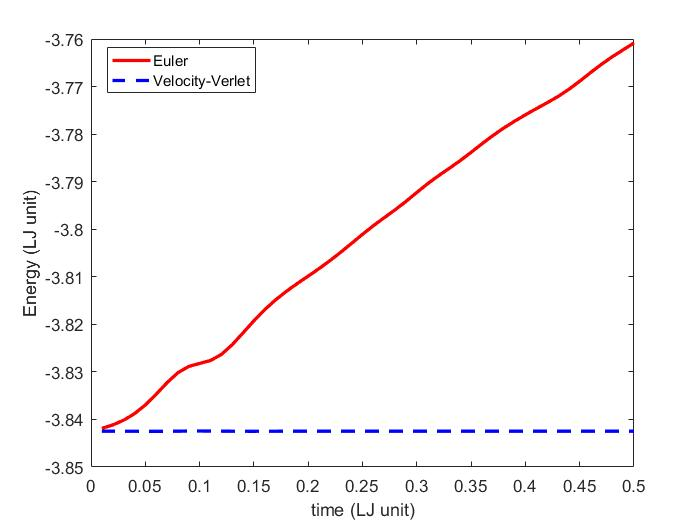
\includegraphics[scale=0.43]{AlgorithmVariants_EnergyPlots.jpg}
	\caption{Comparison of total energy conservation for Euler and Velocity verlet algorithms}
	\end{figure}
	
The code downloaded from the course website was used, which implements the Velocity Verlet algorithm by default. Euler scheme was implemented by modifying the \texttt{SingleStep()} section in the code. The time step was changed to $0.001$, but for all the other parameters, the default values were used from the input file \texttt{md.in}. 

Since the code is rather long and the modifications were minor, just the parts with the numerical schemes are shown below.
	\begin{figure}[!htbp]
	\centering
	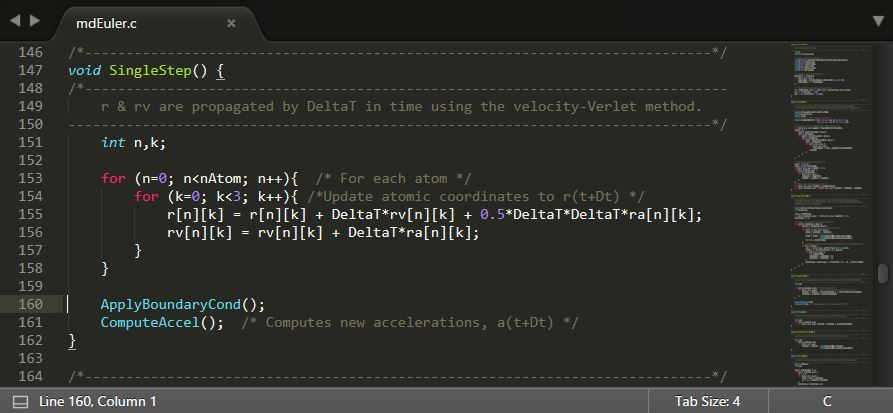
\includegraphics[scale=0.8]{EulerScheme.jpg}
	\caption{Euler scheme implementation}
	\end{figure}
	
	\begin{figure}[!htbp]
	\centering
	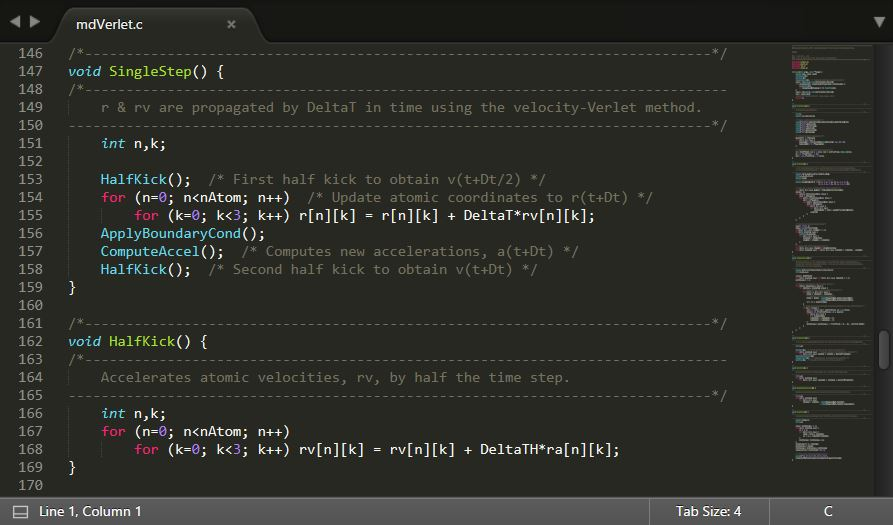
\includegraphics[scale=0.8]{VelVerletScheme.jpg}
	\caption{Euler scheme implementation}
	\end{figure}
	
\section{Velocity Autocorrelation Function}
 Here, we calculate the velocity autocorrelation function
 	\begin{equation}
 	Z(t) = \frac{\langle \vec{v}_i(t+t_0) \cdot \vec{v}_i(t_0) \rangle}{\langle \vec{v}_i(t_0) \cdot \vec{v}_i(t_0) \rangle} = \frac{\sum \limits_{t_0} \sum \limits_{i=1}^N \vec{v}_i(t+t_0) \cdot \vec{v}_i(t_0)}{\sum \limits_{t_0} \sum \limits_{i=1}^N  \vec{v}_i(t_0) \cdot \vec{v}_i(t_0)}
 	\end{equation}
 	where $\vec{v}_i(t)$ is the velocity of the $i$-th atom at time $t$. The bracket denotes averages over
atoms, $i$, and the time origin, $t_0$.

The \texttt{md.c} program from the course website was modified to calculate autocorrelation function. In summary, the \texttt{calc\_vac} function was added to calculate the numerator term of Eqn (6), and some lines were added in the \texttt{main} 
function-- variable \texttt{denm} to accumulate the sums in the denominator term and an outer loop to run the simulation \texttt{NSAMPLE} times and take averages. The required variable were added in the \texttt{md.h} header file, but are not shown here as these additions were not significant. The modified part of the \texttt{md.c} is shown below.
	\begin{figure}[!htbp]
	\centering
	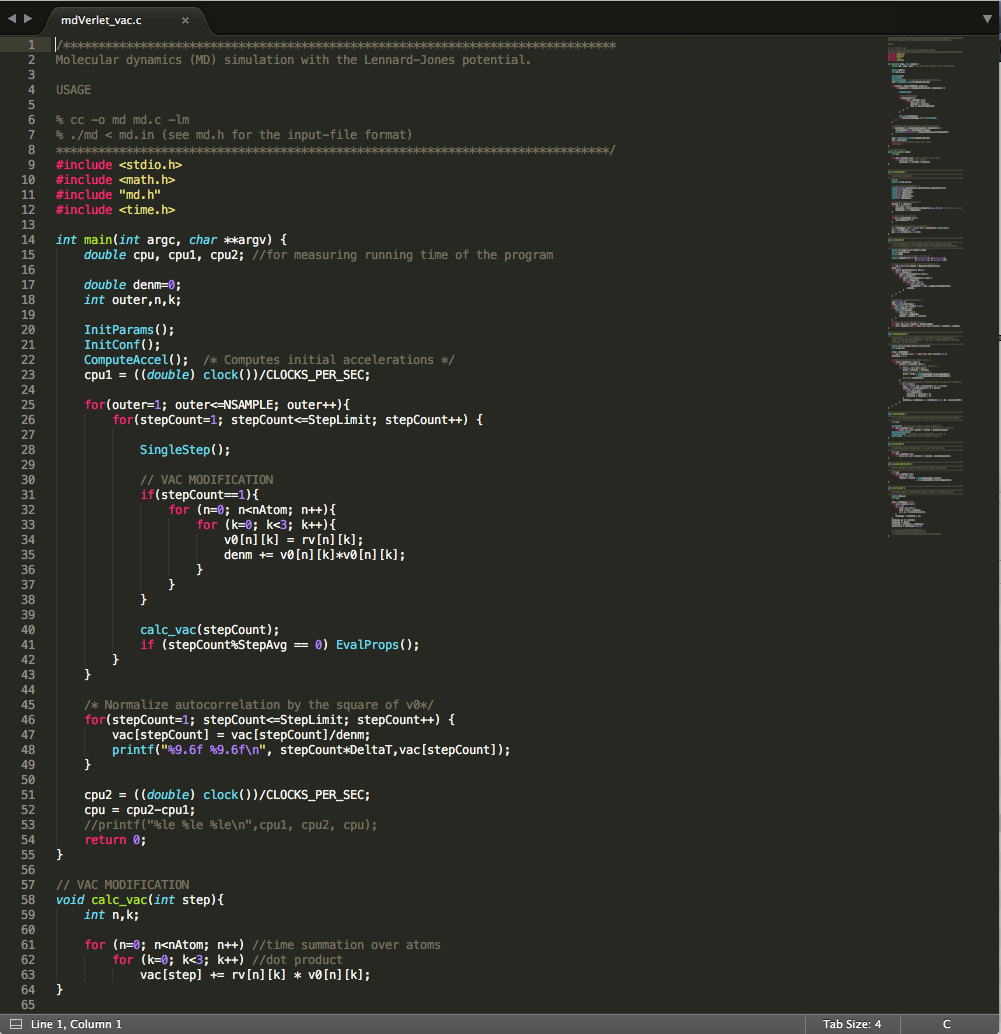
\includegraphics[scale=0.35]{mdVerlet_vac_pic.jpg}
	\caption{Modified Code block}
	\end{figure}

The program was run using \texttt{InitUcell = {3,3,3}, DeltaT = 0.005} and \texttt{StepAvg = 10}, for \texttt{StepLimit = 2000} steps to calculate VAC in the time range of \texttt{[0, tmax = DeltaT*StepLimit = 0.005*2000 = 10.0]} for both gas phase (\texttt{Density = 0.1, InitTemp = 1.0)} and solid phase \texttt{(Density = 1.0, InitTemp = 0.1}). As The results are shown below:
	\begin{figure}[!htbp]
	\centering
		\begin{tabular}{@{}c@{}}
		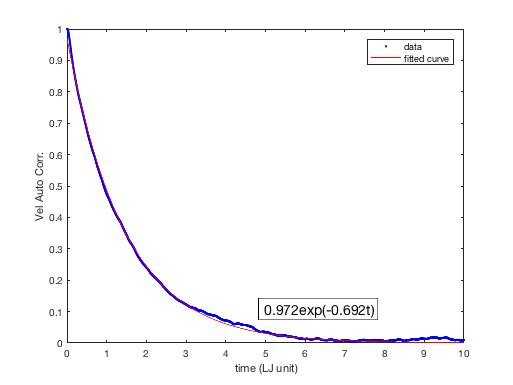
\includegraphics[scale=0.55]{vacGas.jpg} \\[\abovecaptionskip]
		\tiny (a) Velocity autocorrelation vs time for gas phase
		\end{tabular}
		\begin{tabular}{@{}c@{}}
		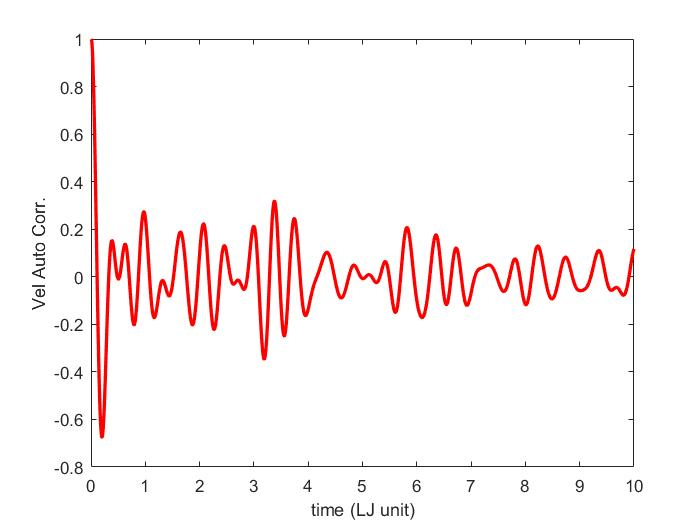
\includegraphics[scale=0.4]{vacSolid} \\[\abovecaptionskip]
		\tiny (b) Velocity autocorrelation vs. time for solid phase
		\end{tabular}
		
	\end{figure}
	
As expected, vac for gas phase dies down from $1$ to $0$ exponentially while for the the solid phase it just fluctuates about zero.
\pagebreak
\section{Split Operator Formalism- Deriving the Velocity Verlet algorithm}
Consider a conservative system of $N$ atoms which can translate along $x$, $y$ and $z$ axes. Hence, the total degrees of freedom of the system are
	\begin{equation}
	f = 3N
	\end{equation}
Let $x$ denote the position, $p$ momentum, and $V$ the potential energy of the system. Then, the Hamiltonian of the system is given by
	\begin{equation}
	H = \sum \limits_{j=1}^N \frac{p_j}{2m} + V(x_1, x_2, ...., x_f)
	\end{equation}
Differentiating the above equation to get $\dot{x}_j$ and $\dot{p}_j$, and noting that the system is conservative,
	\begin{align}
	\dot{x}_j &= \pdv{H}{p_j} = \frac{p_j}{m} \\
	\dot{p}_j &= -\pdv{H}{x_j} = -\pdv{V}{x_j} = F_j
	\end{align}
Now, for any function of the form $\phi(x_1, x_2, ...., x_f, p_1, p_2, ...., p_f)$,
	\begin{align}
	\phi &= \left(\sum \limits_{j=1}^f \dot{x}_j \pdv{}{x}_j + \dot{p}_j \pdv{}{p}_j \right) \phi \\
		&= \underbrace{\left(\sum \limits_{j=1}^f \pdv{H}{p_j} \pdv{}{x}_j + \pdv{H}{x_j} \pdv{}{p}_j \right)}_{\text iL} \phi \\
		&= iL \phi
	\end{align}
where $L$ is defined as the Louiville operator.

Now, consider a special function $\Gamma(x_j, p_j)$ such that,
	\begin{align}
	\frac{d \Gamma}{dt} = iL \Gamma
	\end{align}
This equation integrated to get $\Gamma$.
	\begin{equation}
	\Gamma (t) = \Gamma (0) e^{iLt} 
	\end{equation}
This can be proved as follows. Take the Taylor expansion of the exponential term as follows:
	\begin{equation}
	e^{iLt} = 1 + iLt - \frac{L^2t^2}{2!} -\frac{iL^3 t^3}{3!} + ....
	\end{equation}
Taking the derivative w.r.t $t$,
	\begin{align}
	\frac{d e^{iLt}}{dt} &= iL - L^2t -\frac{iL^3 t^2}{2} + .... \\
				 &= iL \left( 1 + iLt - \frac{L^2t^2}{2!}+ .... \right) \\
				 &= iL e^{iLt}\\
	 \times \Gamma(0), \qquad \qquad  \frac{d (\Gamma(0)e^{iLt})}{dt} &= \Gamma(0) iL e^{iLt} \\
	\therefore \frac{d\Gamma}{dt} &= iL \Gamma
	\end{align}
Let us define the classical propagator as 
	\begin{equation}
	 U(t) = e^{iLt}
	\end{equation}
Note that $U(t)$ is unitary, i.e., $U(-t)  =U(t)$.

Let us now decompose the Louiville operator as follows,
	\begin{align}
	iL &= iL_1 + iL_2 \\
	   &= \underbrace{\sum \limits_j F_j(x_j) \pdv{}{p_j}}_{iL1} + \underbrace{\sum \limits_j\frac{p_j}{m}\pdv{}{x_j}}_{iL2}
	\end{align}
Now, we can write the exponential of the above decomposition using Trotter expansion as
	\begin{align}
	e^{i(L_1 + L_2)t} = (e^{\frac{iL_1 \Delta t}{2}} e^{iL_2 \Delta t} e^{\frac{iL_1 \Delta t}{2}})^P
	\end{align}
where $\Delta t = t/P$. This allows us to define a discrete time propagator as
	\begin{align}
	G(\Delta t) &= U_1(\frac{\Delta t}{2}) U_2(\Delta t) U_1(\frac{\Delta t}{2}) \\
	&= e^{\frac{iL_1 \Delta t}{2}} e^{iL_2 \Delta t} e^{\frac{iL_1 \Delta t}{2}}
	\end{align}
Since we know that $U(t)$ is unitary, it means that $G(\Delta t)$ will also be unitary. Now,let us substitute the definition of the split operators from Eqn (24).
	\begin{equation}
	G(\Delta t) = e^{\Delta t/2 F(x) \pdv{}{p}} e^{ \Delta t \dot{x} \pdv{}{x}} e^{\Delta t/2 F(x) \pdv{}{p}}
	\end{equation}
Operating this on the $\{x(0), p(0) \}$ and using the property for any operator of the form $e^{c \pdv{}{q}}$
	\begin{equation}
	e^{c \pdv{}{q}} f(q) = f(q+c)
	\end{equation}
where $c$ is independent of $q$ (\textit{I don't know how to derive this!}).

Using this, we can derive that
	\begin{align}
	x(\Delta t) &= x(0) + \Delta t \dot{x}(0)+\frac{(\Delta t)^2}{2} \frac{F[x(0)]}{m} \\	
	\dot{x}(\Delta t) &= \dot{x}(0) + \frac{\Delta t}{2m} \{F[x(0)] + F[x(\Delta t] \}
	\end{align}	
which can be written in the known form on the velocity-Verlet algorithm
	\begin{align}
	\dot{x}(\frac{\Delta t}{2}) &= \dot{x}(0) + \frac{\Delta t}{2m} F[x(0)] \\
	x(\Delta t) &= x(0) + \Delta t \dot{x}(\frac{\Delta t}{2}) \\
	\dot{x}(\Delta t) &= \dot{x}(\frac{\Delta t}{2}) + \frac{\Delta t}{2m} F[x(\Delta t)]
	\end{align}

\end{document}